\documentclass{sig-alternate}
\usepackage{float}
\restylefloat{table}

\title{CSCI-620 Data Management with the IMDb Dataset}
\subtitle{[Understanding, modeling, and developing tools to interact with the IMDb dataset]}
\numberofauthors{4}
\author
{
	\alignauthor
	Aishwarya Rao
	\email{ar2711@rit.edu}
	\alignauthor
	Apurav Khare
	\email{ak2816@rit.edu}
	\and
	\alignauthor
	Martin Qian
	\email{jq3513@rit.edu}
	\alignauthor
	Prateek Kalasannavar
	\email{pk6685@rit.edu}
}

\begin{document}
	\maketitle
	\begin{abstract}
		This project aims to explore a dataset by understanding it, modeling it to a normalized relational schema so that it can be stored and retrieved from a relational database management system. The project also focuses on developing an interface that allows fast and easy access to the dataset by abstracting complex query scenarios, like search by specific parameters within and across tables, and aggregate queries.
	\end{abstract}
	
	\section{Project Status}
	As established in Phase 0, the deliverable of Phase 1 includes an entity-relationship diagram of the IMDb dataset based on our exploration and understanding of the dataset structure. This ER diagram is then used to map to a relational schema. These structures have been designed keeping in mind possible query scenarios, ease of access of writing queries as well as fetching results with respect to common requests, and the constraints required to keep ambiguity and inconsistency out of the structure. 
	\subsection{ER Diagram}
	The ER Diagram representing the design of the database is depicted in Figure \ref{ER}
	\begin{figure}[ht]
		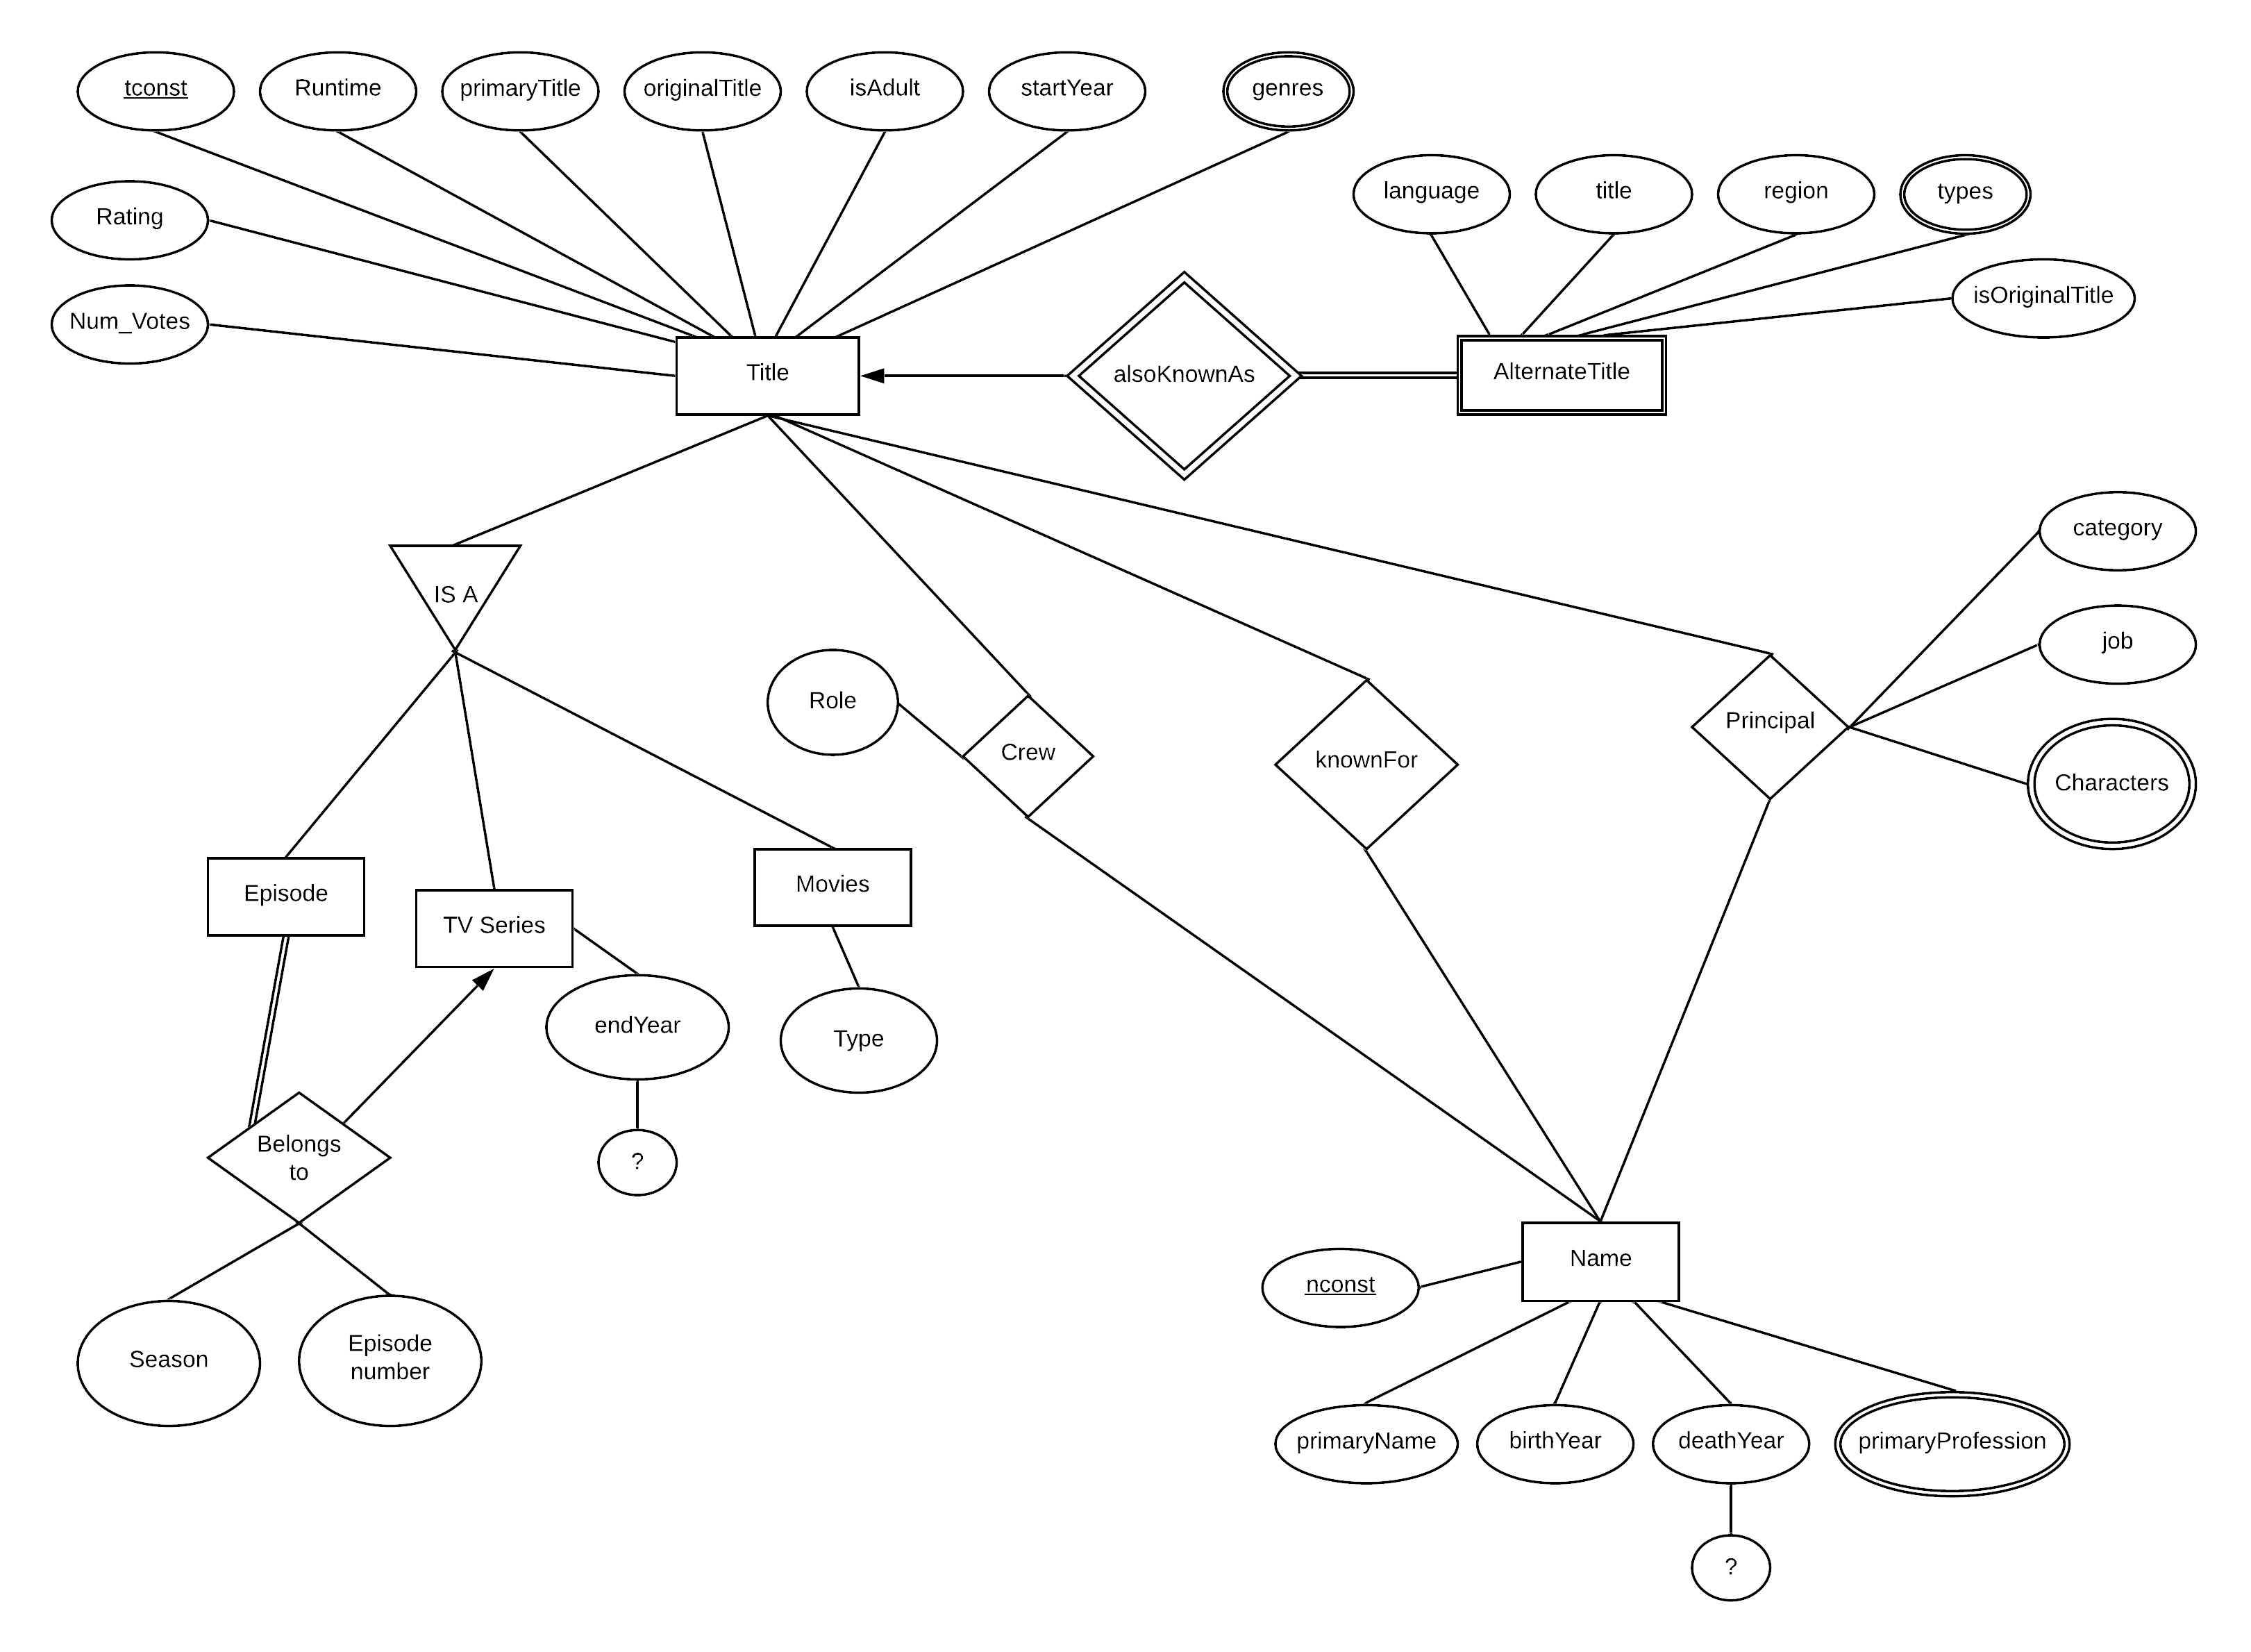
\includegraphics[width=8cm]{er.png}
		\label{ER}
		\centering
	\end{figure}
	The core entity set of the data is the title, which represents a movie or a series or a short. Basic properties that are common among these types are attributes of the title table. To differentiate between movies (which have no episodes) and TV shows, both of whose titles are present in the title table, an IS A relationship is defined. It is assumed that shorts and documentaries are part of movies as they have no separate unique features of their own. Only TV show titles are associated with episode titles with the season and episode number. The rating and the number of votes are considered as attributes of a title since fine-grained information about each review and its rating is not available in the dataset. 
	The other core entity set of the data is the ``name", which refers to the metadata of a person that has participated in a title. Nconst acts as the primary key in this table. 
	A person can have more than one primary profession and hence, this forms a multivalued attribute.
	The relationship between title and a person is in three different forms. One, a person may be a part of the crew for a movie or episode. This job includes producers and writers and are indicated through the role attribute on this relationship. A person may be primarily known for one or more titles. This relationship is captured by known for. Finally, the details regarding the principal team involved in a movie or show (including actors) are represented by a relationship principal that holds the person's role as well as characters they may have played. 
	\subsection{Schema Identification}
	This phase involves the identification and mapping of the relational schema from the entity- relationship Model, as well as choose appropriate constraints and keys required to maintain data integrity and avoid redundancies. The relational schema selected is as follows,\newline
        \begin{itemize}
	\item title (\underline{primaryTitle}, \underline{originalTitle}, \underline{startYear}, isAdult, averageRating, numVotes)
	\item titleGenres (\underline{primaryTitle}, \underline{originalTitle}, \underline{startYear}, \underline{genre}) \newline
	Foreign Key - title(\underline{primaryTitle}, \underline{originalTitle}, \underline{startYear})
	\item tvSeries (\underline{primaryTitle}, \underline{originalTitle}, \underline{startYear}, endYear)\newline
	Foreign Key - title(\underline{primaryTitle}, \underline{originalTitle}, \underline{startYear})
	\item movie (\underline{primaryTitle}, \underline{originalTitle}, \underline{startYear}, \underline{movieType})\newline
	Foreign Key - title(\underline{primaryTitle}, \underline{originalTitle}, \underline{startYear})
	\item tvEpisode (\underline{primaryTitle}, \underline{originalTitle}, \underline{startYear},\\ \underline{seriesPrimaryTitle}, \underline{seriesOriginalTitle}, \underline{seriesStartYear}, \underline{seasonNumber}, \underline{episodeNumber})\newline
	Foreign key 1 - title(\underline{primaryTitle}, \underline{originalTitle}, \underline{startYear})
	Foreign key 2 - tvSeries(\underline{primaryTitle}, \underline{originalTitle}, \underline{startYear})
	\item alternateTitle (\underline{primaryTitle}, \underline{originalTitle}, \underline{startYear},\\ \underline{language}, \underline{title}, \underline{region}) \newline
	Foreign key - title(\underline{primaryTitle}, \underline{originalTitle}, \underline{startYear})
	\item alternateTitleTypes (\underline{primaryTitle}, \underline{originalTitle}, \underline{startYear},\\ \underline{language}, \underline{title}, \underline{region}, \underline{type}) \newline
	Foreign key - title(\underline{primaryTitle}, \underline{originalTitle}, \underline{startYear})
	\item name (\underline{primaryName}, \underline{birthYear}, deathYear)
	\item namePrimaryProfession (\underline{primaryName}, \underline{birthYear},\\ \underline{primaryProfession}) \newline
	Foreign key - name(\underline{primaryName}, \underline{birthYear})
	\item writers (\underline{primaryName}, \underline{birthYear}, \underline{primaryTitle}, \underline{originalTitle}, \underline{startYear}) \newline
	Foreign key 1 - name(\underline{primaryName}, \underline{birthYear}) \newline
	Foreign key 2 - title(\underline{primaryTitle}, \underline{originalTitle}, \underline{startYear})
	\item directors (\underline{primaryName}, \underline{birthYear}, \underline{primaryTitle},\\ \underline{originalTitle}, \underline{startYear}) \newline
	Foreign key 1 - name(\underline{primaryName}, \underline{birthYear}) \newline
	Foreign key 2 - title(\underline{primaryTitle}, \underline{originalTitle}, \underline{startYear})
	\item popularTitles (\underline{primaryTitle}, \underline{originalTitle}, \underline{startYear}, \underline{primaryName}, \underline{birthYear}) \newline
	Foreign key 1 - name(\underline{primaryName}, \underline{birthYear}) \newline
	Foreign key 2 - title(\underline{primaryTitle}, \underline{originalTitle}, \underline{startYear})
	\item principalCast (\underline{primaryTitle}, \underline{originalTitle}, \underline{startYear}, \underline{primaryName}, \underline{birthYear}, \underline{category}, \underline{job}) \newline
	Foreign key 1 - name(\underline{primaryName}, \underline{birthYear}) \newline
	Foreign key 2 - title(\underline{primaryTitle}, \underline{originalTitle}, \underline{startYear})
	\item principalCastCharacters (\underline{primaryTitle}, \underline{originalTitle}, \underline{startYear}, \underline{primaryName}, \underline{birthYear}, \underline{category}, \underline{job},\\ \underline{character}) \newline
	Foreign key - principalCast(\underline{primaryTitle}, \underline{originalTitle}, \underline{startYear}, \underline{primaryName}, \underline{birthYear}, \underline{category}, \underline{job})
        \end{itemize}
	\subsection{Populating the database}
        The database population is done in two steps, to allow for cleaning the data, applying the constraints, and inserting the data.
        \begin{enumerate}
                \item[Step 1:] Create a staging database. The structure of this database is same as the source files. It is used to ease the process of inserting values into the normalized tables. It is created using the file import feature provided by SQL Server. The data in these tables is not sanitized, and doesn't adhere to any constraints.\\
As the tables in the relational schema are in BCNF form, they are decomposed, and can contain values from multiple files to maintain proper functional dependency. Using a staging database allows us to avoid loading multiple large files in the memory to populate a single table. It makes the process of populating the database simpler and cleaner. These tables are created using a Python script that inserts all values from a table into a corresponding table.

                \item[Step 2:] The values are transferred from the staging database to the relational model. For populating each table in the relational schema, the necessary tables from the staging database are joined and the values are converted to a proper type. The data stored in the relational model ensures complete referential integrity and data consistency. This step is done using SQL scripts that read the necessary tables from the staging schema, and populate the tables in the IMDb schema.
        \end{enumerate}
\bigskip
	\section{Project outline}
	The next step of the project is to identify possible scenarios and create queries for the same. Following are some of the query scenarios that we forsee implementing:
        \begin{itemize}
            \item The range of titles released during a specified time period.
            \item Popular titles for a specified actor.
            \item Top list of movies of all time.
            \item Specific movie or actor information based on search.
           \item Aggregated summaries of actors and their contributions to titles.
        \end{itemize}

Simultaneously, a front end interface will be developed for user-friendly access to the results returned by the queries. The user-interface will be web-based, allowing the users to access the data across devices and platforms. The queries to fetch the data for display will be implemented in the back-end REST API that connects to the relational schema created in Phase 1.

The deliverable by the end of this data management project will be the interface that allows users to access and view the data present in the IMDb dataset in a fast and comprehensible way. 
\end{document}